\documentclass[sigconf]{acmart}

% The following packages can be found on http:\\www.ctan.org
\usepackage{tikz}     % For adding axes to plots
\usepackage{graphicx} % For including PDFs
\usetikzlibrary{positioning}
\usepackage{hyperref}


\usepackage{amsmath} % assumes amsmath package installed
\usepackage{amssymb}  % assumes amsmath package installed
\usepackage{textcomp} % For the text tilde low
\usepackage{tabularx}
    \newcolumntype{L}{>{\raggedright\arraybackslash}X}

%% Command for creating multiplie-line cells inside a table environment
\newcommand{\multilinecell}[2][c]{%
  \begin{tabular}[#1]{@{}c@{}}#2\end{tabular}}
  
%% Command for a text tilde
\newcommand{\thomastilde}{\raisebox{0.1ex}{\texttildelow}}

\setcopyright{rightsretained}

% DOI
\acmDOI{}

% ISBN
\acmISBN{}

%Conference
\acmConference[GRAD5134]{Virginia Tech}{Spring, 2018}{Blacksburg, Virginia}
\acmYear{2018}
\copyrightyear{2018}

\keywords{Ethics, Predictive Models, Multilayer Perceptron, Decision Tree, Local}

\begin{document}

\title{Improving the Ethics of Prediction with Interpretable Models}
\titlenote{Authors are listed in alphabetical order by last name. This work was a final project for the Ethics and Professionalism in Data Science Graduate class at Virginia Polytechnic Institute and State University.}

\author{Mohammed Almanaa}
\affiliation{\department{Department of Civil Engineering}}

\author{Reid Bixler}
\affiliation{\department{Department of Computer Science}}

\author{Thomas Lux}
\affiliation{\department{Department of Computer Science}}
 
\author{Stefan Nagy}
\affiliation{\department{Department of Computer Science}}

\author{Sirui Yao}
\affiliation{\department{Department of Computer Science}}


% \thanks{$^{1}$ Student in Department of Civil Engineering}%
% \thanks{$^{2}$ Student in Department of Computer Science}%

% \thispagestyle{empty}
% \pagestyle{empty}

%%%%%%%%%%%%%%%%%%%%%%%%%%%%%%%%%%%%%%%%%%%%%%%%%%%%%%%%%%%%%%%%%%%%%%%%%%%%%%%%
\begin{abstract}
(All members) Large volumes of data allow for modern application of statistical and mathematical models to practical social issues. Many applications of predictive models like criminal activity heatmapping, recidivism estimation, and child safety scoring rely on data that is incomplete, incorrect, or biased. Many sensitive social and historical issues can unintentionally be incorporated into predictions causing ethical mistreatment. This work attempts to address data bias by using models that produce interpretable results. The improvements offered by these models are twofold: (1) bias can be identified either statistically or by human users on a per-prediction basis; (2) data can be cleaned for bias on a per-prediction basis. Modeling techniques similar to those presented in this work could not only strengthen the ethical application of data science, but also make the process of cleaning and validating data manageable in the long term.
\end{abstract}
%%%%%%%%%%%%%%%%%%%%%%%%%%%%%%%%%%%%%%%%%%%%%%%%%%%%%%%%%%%%%%%%%%%%%%%%%%%%%%%%
 
 \maketitle
 
\section{INTRODUCTION (MA)}
\label{sec:introduction}
With the growth of new technologies and machine learning algorithms, smart cities and urban areas are adapting advanced devices to control and monitor many aspects of our life and thus provide better service for our communities and the society as a whole. With the explosion of the massive amounts of collected data (referred to as big data), predictive models have boomed and become an interest for many fields such as healthcare, employment, finance, government \cite{siegel2016predictive}. The predictive models were motivated by the critical need in our daily life to anticipate the future events to prepare and make an action in advance. Succeeding in doing so would stop or mitigate the negative consequences of future events. The predictive models play a role in our daily life, helping us answer various questions, ranging from easy to complicated:\begin{itemize}
\item Do I need to take my umbrella with me when leaving home? 
\item How long will take me to get home/work?
\item How likely this applicant would succeed in the college and thus deserves to be accepted?
\item How likely a criminal defendant would not commit a crime again and thus should be released?
\end{itemize}

The significant increase of the collected data has pushed researchers and agencies in developing very accurate predictive models but not paying much attention to the ethical aspects of the models. Non-Ethical models (i.e. biased models) could lead to treat people differently based on race, color, sex, or religion which is prohibited by the U.S. federal laws. That happens when human subjects are involved in the model such as criminal risk assessment tool.

Ignoring the bias in the predictive models may create serious discriminatory consequences. Many researchers have shown clear signs of unequal and racial treatment of individuals \cite{squires2003racial,stoll2004black,angwinmachine}.  For example, Angwin et al. analyzed a well-known criminal risk assessment: COMPAS and concluded the outcomes of the model are racially biased \cite{angwinmachine}. They showed that ''Black defendants were twice as likely as white defendants to be misclassified as a higher risk of violent recidivism, and white recidivists were misclassified as low risk 63.2 percent more often than black defendants'' . The U.S. government realized the enormous potential for negative impact of the biased predictive models and thus the White House published several reports, highlighting the potential bias that could affect adversely individuals or groups \cite{smith2016big}. Research efforts have been conducting actively in proposing ethical frameworks and potential solutions to protect principles of ethics and privacy \cite{dedeo2014wrong,vayena2016elements,kass2001ethics}.

Not-ethical models do not necessarily mean they contain personal characteristics as predictors, yet they could impose racial bias, for instance, if they have other predictors correlated with race. This makes developing unbiased models harder given the researchers have to dig deep into the results, making sure the bias is not existed, and thus there is a need to use models that produce interpretable results. That could make it possible for a researcher to detect the bias before making prediction.

In this paper, we attempt to address data bias by using models that produce interpretable results. The improvements offered by these models are twofold: (1) bias can be identified either statistically or by human users on a per-prediction basis; (2) data can be cleaned for bias on a per-prediction basis. Modeling techniques similar to those presented in this work could not only strengthen the ethical application of data science, but also make the process of cleaning and validating data manageable in the long term.

\subsection{Ethical Violation: Recovering Protected Information}

In an effort to prevent biased and discriminatory decisions, policy makers and practitioners have classified discriminatory attributes such as personal attributes as protected information and thus cannot be used as predictors in the model. However, researchers have shown this approach is inadequate as the discrimination and biases are still existed (i.e. indirect bias), and more importantly, protected information can be easily recovered \cite{dedeo2014wrong,pedreshi2008discrimination}. Pedreschi et al. have shown that discrimination rules could be inferred using protected German credit dataset. This was done by linking the outcomes of the model (i.e. discrimination rules) with other background knowledge. For instance, knowing there is a majority of black people living in this neighborhood means any resultant classification  rules are linked with black people. Dedeo showed the existing correlation between protected and non-protected variables made it possible for unveiling the protected information \cite{dedeo2014wrong}. They proposed one approach to overcome this issue by de-correlating category and outcome using the Information Theory.

\subsection{Global Predictive Models}
Classic machine learning and data science techniques applied today often rely on solving a very specific problem. They create a global predictive model with the aim of capturing trends that exist across thousands of examples. In general, these global models are constructed given data matrix $X \in \mathbb{R}^{n\ \times\ d}$, a truth function $f: \mathbb{R}^d \rightarrow \mathbb{R}$, and \textit{labels} $f(x^{(i)})$ for row vectors $x^{(i)} \in X$, $1 \leq i \leq n$. These models find the solution to

$$ \min_P \bigl\|\ \hat f_P(X) - f(X)\ \bigr\|, $$

where $\hat f_P: \mathbb{R}^d \rightarrow \mathbb{R}$ is the parametric approximation, $f(X)$ is used to denote the vector with components $f(X)_i = f(x^{(i)})$, and $\| \cdot \|$ is an appropriate measure. The labels may be real numbers, like probability of recidivism estimates, or categories such as "safe" or "not safe" for an at-risk child.

The difficulty with these models is that the minimization search which identifies the parameters for the model is performed over \textit{all} data. Whenever it is time to explain a prediction, the answer is often "all data was used to capture this trend". The models of this form that will be applied are a multilayer perceptron (MLP) and a decision tree (DT).

\subsubsection{Multilayer Perceptron}

The neural network is a well studied and widely used method for both regression and classification tasks \cite{hornik1989multilayer}. When using the rectified linear unit (ReLU) activation function \cite{dahl2013improving} and training with the BFGS minimization technique \cite{moller1993scaled}, the model built by a multilayer perceptron uses layers $l : \mathbb{R}^{i} \rightarrow \mathbb{R}^{j}$ defined by

$$ l(u) = \big( u^t W_l \big)_+ ,$$

where $W_l$ is the $i$ by $j$ weight matrix for layer $l$. In this form, the multilayer perceptron produces a piecewise linear model of the input data. The computational complexity of training a multilayer perceptron is $\mathcal{O}(n d m)$, where $m$ is determined by the sizes of the layers of the network and the stopping criterion of the BFGS minimization used for finding weights. This paper uses the scikit-learn MLP regressor \cite{scikit-learn}, a single hidden layer with 100 nodes, ReLU activation, and BFGS for training.

\subsubsection{Decision Tree}

The decision tree is used because of the relatively straightforward interpretation of the prediction process. Model construction is out of the scope of this description, but is a well-studied process \cite{quinlan1986induction}. A prediction at a point $z \in \mathbb{R}^d$ for a decision tree constructed over a real vector space is made by traversing nested axis-aligned conditionals of the form
$$\hat f(z) = \hat f(z | z_{k^{(1)}} \geq v^{(1)}, \ldots) $$

This paper uses the scikit-learn Decision Tree regressor \cite{scikit-learn}, no maximum depth or number of nodes, and the Gini impurity measure of information gain.

\subsection{Local Predictive Models}

The construction of approximation functions $\hat f_P: \mathbb{R}^d \rightarrow \mathbb{R}$ as described for global models can instead be approached on a per-prediction basis. A model is henceforth referred to as \textit{local} when any prediction made at a point $z \in \mathbb{R}^d$ is only a function of a set of points $L \subset X$, where membership in $L$ is determined by a distance metric. The advantage of using a local model is a more compact description of \textit{how} a prediction is made that is derived from a manageable subset of all known data. \textit{Local} models become particularly useful when predictions regard ethically sensitive issues and need to be rigorously evaluated for bias. The source data for any prediction can be checked on the spot for fairness of representation against any number of protected attributes.

The following sections describe the three local approximation techniques that will be used to predict recidivism likelihood in this work.

\subsubsection{Nearest Neighbor}

This algorithm will be used as a baseline for comparison because it is the most mathematically simple \textit{local} model in this study. A prediction is made for Nearest Neighbor at point $z \in \mathbb{R}^d$ by
$$ \hat f(z) = f \big ( \text{\textit{argmin}}_{x^{(i)} \in X} \| z - x^{(i)} \|_2 \big). $$
This approximation technique can be applied in a wide range of applications, however it must be noted that the approximation surface it produces is not $C^0$ (continuous in value).

% Local models have gained attention due to their flexibility and ability to capture underlying changes over time, offering a powerful tool for many applications in different fields \cite{west1985dynamic}. Unlike other statistical and batch machine learning algorithms models, the local models estimation and forecasting can be done recursively without a need to store the entire past history. Given the available information, they adapt themselves in a very short time as new data arrive, outperforming many advanced algorithms. In addition, local models inference and prediction can efficiently handle the missing data problem.

% Almost all machine learning algorithms can be treated local models in which we use solely a fixed-length moving time window for training. This step would make the computational time smaller, giving us a great chance to apply it on online complex problems that cannot handle any delay in the prediction. Yet, this approach would not be ideal if there is a core knowledge that cannot be discovered without running the entire dataset.



\subsubsection{Delaunay Triangulation}

The Delaunay method of interpolation is a well studied geometric technique for producing an interpolant \cite{lee1980two}. The Delaunay triangulation of a set of data points into simplices is such that the sphere defined by the vertices of each simplex contains no data points in the sphere's interior. For a $d$-simplex S with vertices $v^{(0)}$, $v^{(1)}$, $\ldots$, $v^{(d)}$, $x \in S$, and data values $f(v^{(i)})$, $i=0$, $\ldots$, $d$, $x$ is a unique convex combination of the vertices,

$$ x = \sum_{i=0}^{d} w_i v^{(i)}, \quad \sum_{i=0}^{d} w_i = 1, \quad
w_i \geq 0, \quad i=0,\ldots,d ,$$

and the Delaunay interpolant to $f$ at $x$ is given by

$$ p(x) = \sum_{i=0}^{d} w_i f(v^{(i)}). $$

The computational complexity of the Delaunay triangulation (for the implementation used here) is $\mathcal{O} O(n^{1+\frac{1}{d}} d^{3} + n d^{4})$ per prediction, which should reasonably scale to $d < 100$. A newly released Fortran implementation of this polynomial-time Delaunay interpolation technique is used here \cite{chang2018polynomial}.

\subsubsection{Voronoi Mesh}

The final of the three meshes utilizes 2-norm distances to define boundaries rather than max norm distances. A well-studied technique for classification and approximation is the nearest neighbor algorithm \cite{cover1967nearest}. Nearest neighbor inherently utilizes the convex region $v^{x^{(i)}}$ (Voronoi cell \cite{dirichlet1850reduction}) consisting of all points closer to $x^{(i)}$ than any other point $x^{(j)}$. The Voronoi mesh smooths the nearest neighbor approximation by utilizing the Voronoi cells to define support via a generic basis function $V: \mathbb{R}^d \rightarrow \mathbb{R}_+$ given by

$$ V^{x^{(i)}}(y) = \left(1 - \frac{\bigl\|y - x^{(i)}\bigr\|_2}{2 \ d(y \mid x^{(i)})} \right)_+, $$
where $x^{(i)}$ is the center of the Voronoi cell, $y \in \mathbb{R}^d$ is an interpolation point, and $d(y \mid x^{(i)})$ is the distance between $x^{(i)}$ and the boundary of the Voronoi cell $v^{x^{(i)}}$ in the direction $y - x^{(i)}$. $V^{x^{(i)}}\bigl(x^{(j)}\bigr) = \delta_{ij}$ and $V^{x^{(i)}}$ has local support. While $V^{x^{(i)}}(x^{(i)}) = 1$, the $2$ in the denominator causes all basis functions to go linearly to $0$ at the boundary of the twice-expanded Voronoi cell. Note that this basis function is $C^0$ because the boundaries of the Voronoi cell are $C^0$. In the case that there is no boundary along the vector $w$, the basis function value is always $1$.

While the cost of computing the exact Voronoi cells for any given set of points grows exponentially \cite{dutour2009complexity}, the calculation of $d$ is linear with respect to the number of control points and dimensions. Given any center $x^{(i)} \in \mathbb{R}^d$, set of control points $C \subseteq X$, and interpolation point $y \in \mathbb{R}^d$, $d\bigl(y \mid x^{(i)}\bigr)$ is the solution to
$$
  \max_{c \in C\backslash\{x^{(i)}\}} \frac{\bigl\|y - x^{(i)}\bigr\|_2}{2} \ \frac{y \cdot \bigl(c - x^{(i)}\bigr) - x^{(i)} \cdot \bigl(c - x^{(i)}\bigr)}{c \cdot \bigl(c - x^{(i)}\bigr) - x^{(i)} \cdot \bigl(c - x^{(i)}\bigr)}.
$$



%% ===================================================================

\section{RELATED WORK (SN)}
\label{sec:related}
Algorithmic bias has long been a subject of research on machine learning \cite{kirkpatrick2016battling, hajian2016algorithmic, baeza2016data}. 
Mitchell \cite{mitchell1980need} initially defined machine learning bias as ``any basis for choosing one generalization over another, other than strict consistency with the instances''.
Mooney \cite{mooney1996comparative} expanded this definition with the following assertions: (1) that every model bears some inherent bias, and (2) that detecting a model's bias requires comparison against others.
In recent years, the broad adoption of machine learning has made algorithmic bias a factor in real-world data discrimation \cite{squires2003racial, stoll2004black, angwinmachine}.

Several prior works have explored the problem of measuring algorithmic bias \cite{romei2014multidisciplinary, kamiran2013quantifying, zliobaite2015survey}.
Calders \& Verwer \cite{Calders2010} formalized discrimination as, given an input characteristic, the unequal distribution of outputs for different groups. 
Calders-Verwer (CV) scoring is frequently \cite{kamishima2011fairness, kamishima2012fairness, galhotra2017fairness, calders2009building, kamiran2009classifying, kamiran2010discrimination, kamiran2012decision, vzliobaite2011handling} used to measure \emph{group discrimation} \cite{zafar2015learning, zemel2013learning}. For example, if a loan classifier produces dissimilar outcomes for both sexes (e.g. $P(Y=loan|S=male) > P(Y=loan|S=female)$), then its CV score is measured as the difference in outcomes between those groups (e.g. $P(Y=loan|S=male) - P(Y=loan|S=female)$.
Many works have since expanded on CV scoring for preventing discrimination \cite{hajian2011discrimination, vzliobaite2011handling, zafar2017fairness, kamiran2010discrimination, kamiran2013techniques, galhotra2017fairness}. 
Four general approaches exist: (1) \emph{Suppression} -- removing attributes most correlating with discrimination-sensitive attributes; (2) \emph{Dataset ``massaging''} -- altering labels of some objects to mitigate unwanted classifier outcomes; (3) \emph{Reweighting} -- assigning data carefully chosen weights to lessen the degree of discrimination; (4) \emph{Sampling} -- under- and over-sampling certain groups to compensate.

A recent focus of machine learning and data science research has been on improving model interpretability \cite{lipton2016mythos, juang2013data, zhou2008low}.
More specific goals include transparency for assessing model ethicacy \cite{goodman2017european, herman2017data}, augmenting informativeness \cite{kim2015interactive, yang2018visually, wu2017interpretable}, and inferring causality \cite{wang1999smoking, briand1993developing, syed2009enzyme}. 
An obstacle to model interpretability is the lack of transparency of black-box classifiers such as deep neural networks \cite{casillas2013interpretability, cortez2013using, krause2016interacting}.  Post-hoc interpretability \cite{lipton2016mythos} (e.g. visualizations or explanations) represents a promising alternative, however, formalizing  ``model-agnostic'' methodologies remains an ongoing research problem \cite{ribeiro2016should}.

%% ===================================================================

\section{DATA (SY)}
\label{sec:data}
We are using the 3-Year Recidivism for Offenders Released from Prison dataset, publicly available on the webpage of U.S. Government’s open data (data.gov). This dataset reports whether an offender is re-admitted to prison or not within three years from being released from prison. With this dataset, we could either perform a classification task (predict whether or not a released offender would recidivate), or a regression task (predict the probability of recidivism), for the latter, we collapse all identical instances to one and approximate the probability of recidivism with the frequency of positive instances.

We first computed simple statistics on the dataset so that we are aware of the imbalance and discrepancies in the dataset that could lead to bias. This dataset provides $21,646$ instances, Among which $14,619$ instances are negative and $7,027$ instances are positive. We also computed the population across ethinicity groups and compared it against the actual population breakdown by race in Iowa in 2016 (See figure \ref{fig:mesh1}), we noticed that there exist obvious gaps especially for White non-hispanic (dataset: $67.4\%$, actual population: $88.7\%$) and Black or African American (Dataset: $23.6\%$, actual population: $2.9\%$). 

\begin{figure}
  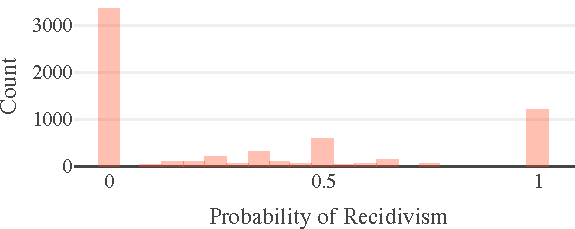
\includegraphics[width=.48\textwidth]{regression_values_histogram.pdf}
  \caption{A 20-bin histogram of the values for recidivism likelihood in the regression task composed of 6,632 samples.}
  \label{fig:histogram_of_recidivism}
\end{figure}

\begin{figure}
    \centering
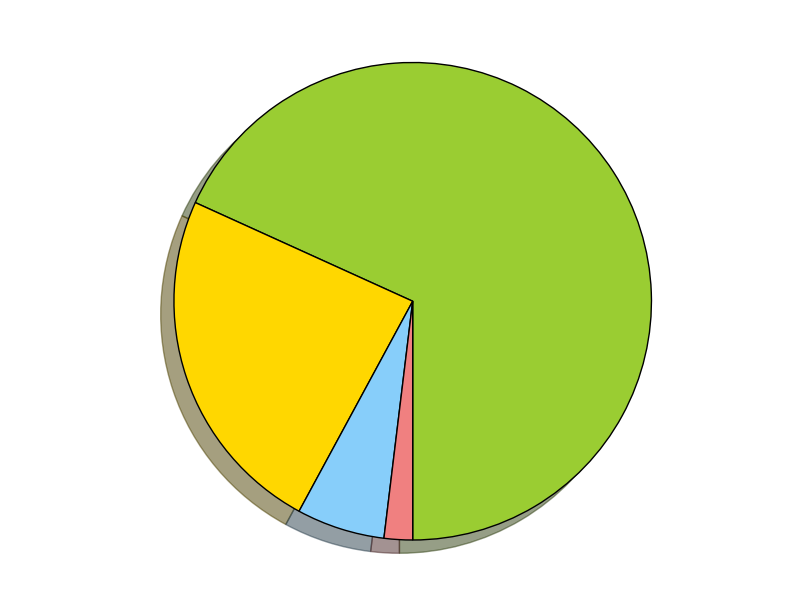
\includegraphics[scale=0.2]{figure_2.png}
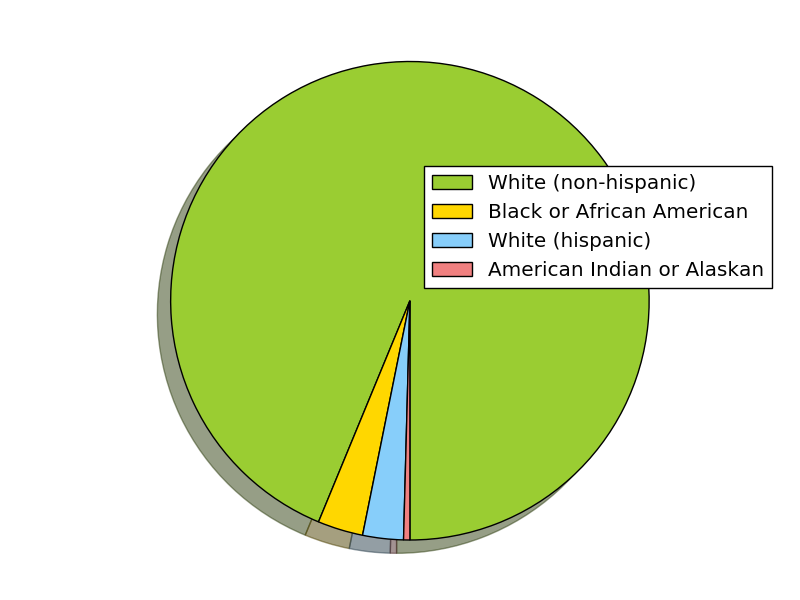
\includegraphics[scale=0.2]{figure_1.png}
    \caption{The distribution across ethnicity groups of the dataset (left) and the actual population in Iowa (right)}
    \label{fig:mesh1}
\end{figure}



Next we preprocessed the features. Each instance in the dataset is described with 16 features and a label indicating whether this prisoner recidivates. First of all, 6 of these features are used to describe the new crime if recidivisms occurs and are therefore unavailable for the negative instances, so we exclude these features; Second, 	we found that two features can be easily computed or inferred from other predictors, specifically, "Recidivism Reporting Year" is always three years later than "Fiscal Year Released", and "Convicting Offense Type" can be uniquely identified with "Convicting Offense Subtype", so we removed these two features. Third, "Race - Ethnicity" is reserved as protected attribute and is later used to evaluate biases in predictions. Therefore, we have 7 features left and we removed the instances that have empty entries for the selected features. Specifically, the 7 features are:
\begin{itemize}
\item Fiscal Year Released
\item Sex
\item Age At Release
\item Convicting Offense Classification
\item Convicting Offense Subtype
\item Release Type
\item Main Supervising District
\end{itemize}

\begin{table*}
\begin{center}
\begin{tabular}{ c | c }
 \hline
 \textbf{FEATURE NAME} & \textbf{VALUES} \\
 \hline
 Sex & F, M \\
  \hline
 Age At Release & Under 25, 25-34, 35-44, 45-54, 55 and Older \\  
  \hline
 Convicting Offense Classification & Aggravated Misdemeanor, Serious Misdemeanor, Sexual Predator Community Supervision, etc \\
  \hline
Convicting Offense Subtype & Murder, Alcohol, Weapons, Drug Possession, Assault, Traffic, Burglary, Forgery/Fraud, Animals, Theft, etc\\  
 \hline
Release Type & Special Sentence, Parole Granted, Discharged - Expiration of Sentence, Released to Special Sentence, etc \\  
 \hline
Main Supervising District & 1JD, 2JD, 3JD, 4JD, 5JD, etc\\  
 \hline
\end{tabular}
\end{center}
\caption{Sample values of categorical features selected}
\label{table:1}
\end{table*}

Except "Fiscal Year Released", all attributes are categorical. We show some sample values of these categorical features in table \ref{table:1}. We discard any categories with less than 100 samples in order to reduce the resulting dimension and prevent predictions from being made with statistically insignificant amounts of supporting data. We encode categorical features with $c$ unique categories into $\mathbb{R}^{c-1}$ by mapping each category onto one of the vertices of a regular simplex centered at 0 where all vertices $v$ satisfy $\|v\|_2 = 1$. We also consider representing "Age At Release" categories using their average ages, to reduce the number of dimensions in input space. 

Finally, in our experiments, predictions are evaluated against the labels, race \& ethnicity information are used to evaluate model bias. With all the processing, we have 21,018 instances in a 50 dimensional space for classification; for regression, since all identical instances are represented with one, the number of instances drop to 6,632 and the distribution of the response values can be seen in figure \ref{fig:histogram_of_recidivism}.




% $\ $
% \\ \{ What data are we using? \}
% \\ \{ What are its features, how big is it? \}
% \\ \{ What are the protected fields? \}
% \\ $\ $


% \begin{table*}
%   \centering
%   \begin{tabular}{c|c}
%     \hline
%     \textbf{Feature} & \textbf{Categories}\\
%     \hline
%     Fiscal Year Released & \multilinecell{2010, 2011, 2012, 2013, 2014}\\
%     \hline
%     Recidivism Reporting Year & \multilinecell{2013, 2014, 2015, 2016, 2017}\\
%     \hline
%     Sex & F, M\\
%     \hline
%     Age At Release & \multilinecell{Under 25, 25-34, 35-44, 45-54, 55 and Older}\\
%     \hline
% %     Convicting Offense Classification & Aggravated Misdemeanor, Special Sentence 2005, Serious Misdemeanor, B Felony, Other Felony (Old Code), A Felony, Convicting Offense Classification, C Felony, Sexual Predator Community Supervision, Felony - Enhanced, D Felony, Simple Misdemeanor, Felony - Mandatory Minimum, Felony - Enhancement to Original Penalty, Other Felony\\
% %     \hline
%   \end{tabular}
%   \caption{Describe me
%     \vspace{-.5cm}}
%   \label{tab:data_description}
% \end{table*}

% \begin{figure}
%   \includegraphics[width=.5\textwidth]{name.pdf}
%   \caption{Describe me
%   \vspace{-.5cm}}
%   \label{}
% \end{figure}

%% ===================================================================

\section{RESULTS (TL)}
\label{sec:results}

The nearest neighbor (baseline), neural network, and decision tree are applied to both the classification and regression tasks. The Delaunay and Voronoi mesh interpolants are only applied to the regression task. First we analyze the classification results on the raw data. In order to best estimate the real-world performance of these algorithms, \textit{k-fold} cross validation as described in \cite{kohavi1995study} with $k=10$ is used. All algorithms are given the same ten folds of randomized training and testing data in order to maintain comparative fairness. Note that in this scheme there will be exactly one prediction made for each data point, meaning all analysis of results is done with the same sized data as described in Section \ref{sec:data}.

\begin{figure}
  \centering
  
  % Nearest neighbor
  \begin{tabular}{c c}
    \vspace{3mm} \\
    \multicolumn{2}{c}{\textit{NearestNeighbor}} \\
    \vspace{-2mm} \\
    \begin{tabular}{c c c}
      & GN & GR \\ \cline{2-3}
      TN & \multicolumn{1}{|c|}{47.6\%} & \multicolumn{1}{|c|}{19.8\%} \\ \cline{2-3}
      TR & \multicolumn{1}{|c|}{20.1\%} & \multicolumn{1}{|c|}{12.5\%} \\ \cline{2-3}
       & & \vspace{-2mm} \\
      \multicolumn{3}{r}{Accuracy: 60.1\%} \\
    \end{tabular} & 
    \begin{tabular}{|c l|}
      \hline
      20.6\% & White - NH \\
      19.8\% & Black - NH \\
      17.2\% & White - H \\
      16.3\% & AI or NA \\
      20.7\% & Asian or PI \\
      \hline
    \end{tabular} \\
  \end{tabular}
 
  % Decision tree
    \begin{tabular}{c c}
    \vspace{3mm} \\
    \multicolumn{2}{c}{\textit{DecisionTreeClassifier}} \\
    \vspace{-2mm} \\
    \begin{tabular}{c c c}
      & GN & GR \\ \cline{2-3}
      TN & \multicolumn{1}{|c|}{55.8\%} & \multicolumn{1}{|c|}{11.6\%} \\ \cline{2-3}
      TR & \multicolumn{1}{|c|}{23.6\%} & \multicolumn{1}{|c|}{9.0\%} \\ \cline{2-3}
       & & \vspace{-2mm} \\
      \multicolumn{3}{r}{Accuracy: 64.8\%} \\
    \end{tabular} & 
    \begin{tabular}{|c l|}
      \hline
      11.2\% & White - NH \\
      12.1\% & Black - NH \\
      8.7\% & White - H \\
      7.9\% & AI or NA \\
      12.7\% & Asian or PI \\
      \hline
    \end{tabular} \\
  \end{tabular}

  % Neural network
  \begin{tabular}{c c}
    \vspace{3mm} \\
    \multicolumn{2}{c}{\textit{MLPClassifier}} \\
    \vspace{-2mm} \\
    \begin{tabular}{c c c}
      & GN & GR \\ \cline{2-3}
      TN & \multicolumn{1}{|c|}{59.7\%} & \multicolumn{1}{|c|}{7.8\%} \\ \cline{2-3}
      TR & \multicolumn{1}{|c|}{24.5\%} & \multicolumn{1}{|c|}{8.1\%} \\ \cline{2-3}
       & & \vspace{-2mm} \\
      \multicolumn{3}{r}{Accuracy: 67.7\%} \\
    \end{tabular} & 
    \begin{tabular}{|c l|}
      \hline
      7.9\% & White - NH \\
      8.0\% & Black - NH \\
      5.2\% & White - H \\
      3.6\% & AI or NA \\
      9.3\% & Asian or PI \\
      \hline
    \end{tabular} \\
  \end{tabular}
  \vspace{3mm}
  \caption{Performance of three of the algorithms on the classification problem. Left column represents the confusion matrices with rows "true no recidivism" (TN), "true recidivism" (TR), and columns "guessed no recidivism" (GN), "guessed recidivism" (GR). The right column represents the false positive rate for predicting recidivism broken down by race. The race category abbreviations are: not Hispanic (NH), Hispanic (H), American Indian (AI), Native Alaskan (NA), and Pacific Islander (PI).}
  \label{fig:classification_performance}
\end{figure}

In figure \ref{fig:classification_performance} we see the initial results on the classification task of predicting whether or not an admitted prisoner will recidivate upon release. The overall top performer by accuracy is the multilayer perceptron, but it also has the highest false negative prediction rate and the largest discrepancy in false positives by race ("positive" refers to recidivism). Generally it would be expected that any racial crime correlations present would be largest for the race which makes up the largest percentage of data. Interestingly that trend is not observed with the racial outcomes. Larger false positive rates were attributed occasionally to the least represented races (AI or NA, Asian or PI) and also the most represented race (White - NH). It should be noted that the \textit{explanation} for predictions made by the decision tree and multilayer perceptron must be provided in the context of all data. For ethical applications, it may be concerning that the racial representation of the prison data does not match the distribution of the population of the state of Iowa (presuming there is the potential for racial discrimination in historical criminal sentencing).

\begin{figure*}
\centering
\begin{tabular}{l r}

  % NearestNeighbor
  \begin{tabular}{c c}
    \vspace{3mm} \\
    \multicolumn{2}{c}{\textit{NearestNeighbor}} \\
    \multicolumn{2}{c}{ 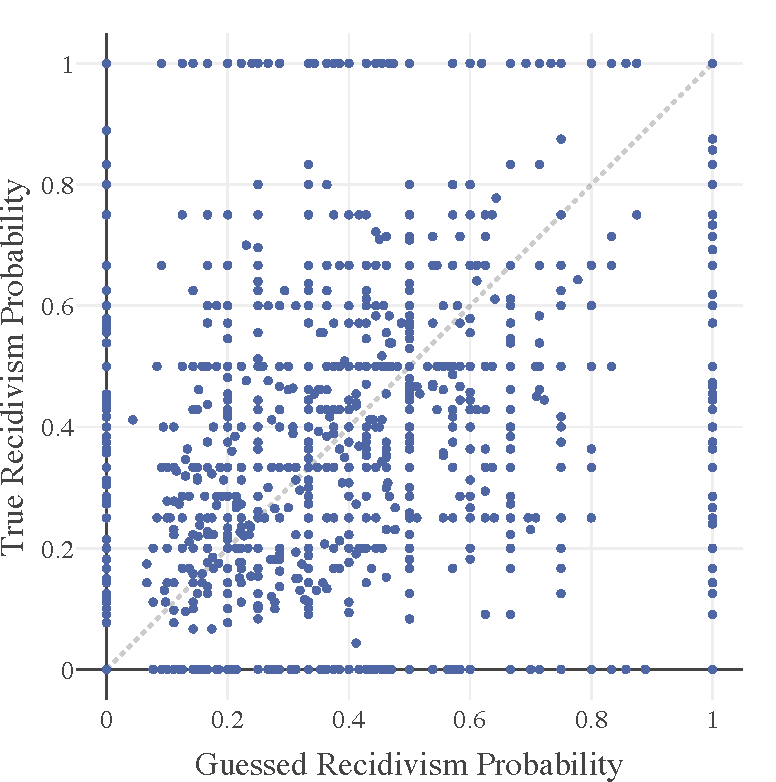
\includegraphics[width=2in,height=2in]{NearestNeighbor_regression.pdf}} \vspace{3mm} \\
    \begin{tabular}{c|c}
        Min & 0.000 \\
        $25^{th}$ & 0.033 \\
        $50^{th}$ & 0.167 \\
        $75^{th}$ & 0.400 \\
        Max & 1.000 \\
    \end{tabular} &
    \begin{tabular}{|c l|}
      \hline
      0.226 & White - NH \\
      0.250 & Black - NH \\
      0.200 & White - H \\
      0.167 & AI or NA \\
      0.306 & Asian or PI \\
      \hline
    \end{tabular} \vspace{3mm} \\
  \end{tabular}

  &

  % VoronoiMesh
  \begin{tabular}{c c}
    \vspace{3mm} \\
    \multicolumn{2}{c}{\textit{VoronoiMesh}} \\
    \multicolumn{2}{c}{ 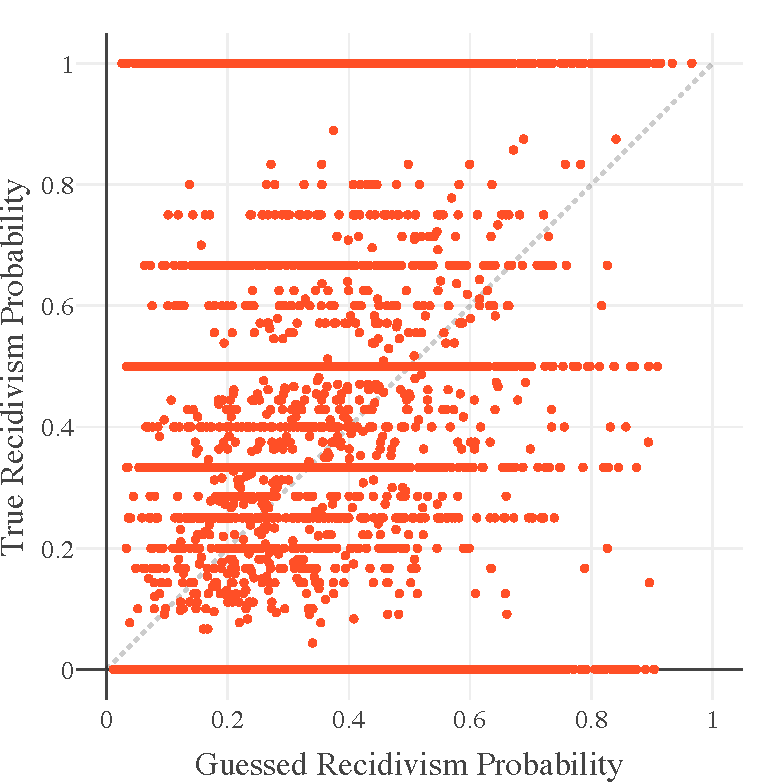
\includegraphics[width=2in,height=2in]{VoronoiMesh_regression.pdf}} \vspace{3mm} \\
    \begin{tabular}{c|c}
        Min & 0.000 \\
        $25^{th}$ & 0.072 \\
        $50^{th}$ & 0.156 \\
        $75^{th}$ & 0.291 \\
        Max & 0.974 \\
    \end{tabular} &
    \begin{tabular}{|c l|}
      \hline
      0.148 & White - NH \\
      0.161 & Black - NH \\
      0.125 & White - H \\
      0.129 & AI or NA \\
      0.139 & Asian or PI \\
      \hline
    \end{tabular} \vspace{3mm} \\
  \end{tabular}

  \\

  % DecisionTreeRegressor
  \begin{tabular}{c c}
    \vspace{3mm} \\
    \multicolumn{2}{c}{\textit{DecisionTreeRegressor}} \\
    \multicolumn{2}{c}{ 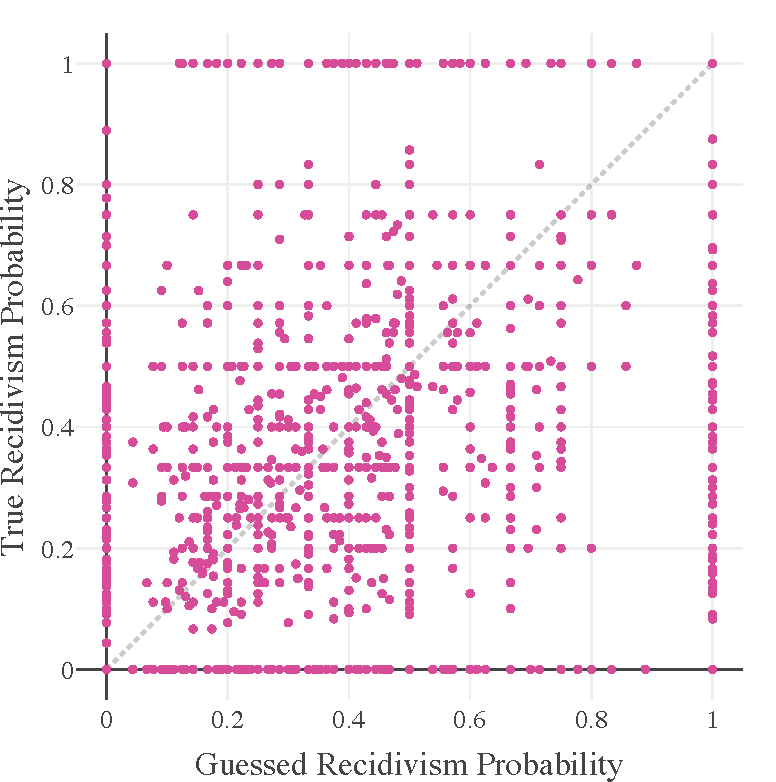
\includegraphics[width=2in,height=2in]{DecisionTreeRegressor_regression.pdf}} \vspace{3mm} \\
    \begin{tabular}{c|c}
        Min & 0.000 \\
        $25^{th}$ & 0.040 \\
        $50^{th}$ & 0.187 \\
        $75^{th}$ & 0.433 \\
        Max & 1.000 \\
    \end{tabular} &
    \begin{tabular}{|c l|}
      \hline
      0.250 & White - NH \\
      0.286 & Black - NH \\
      0.246 & White - H \\
      0.264 & AI or NA \\
      0.257 & Asian or PI \\
      \hline
    \end{tabular} \vspace{3mm} \\
  \end{tabular}

  &

  % MLPRegressor
  \begin{tabular}{c c}
    \vspace{3mm} \\
    \multicolumn{2}{c}{\textit{MLPRegressor}} \\
    \multicolumn{2}{c}{ 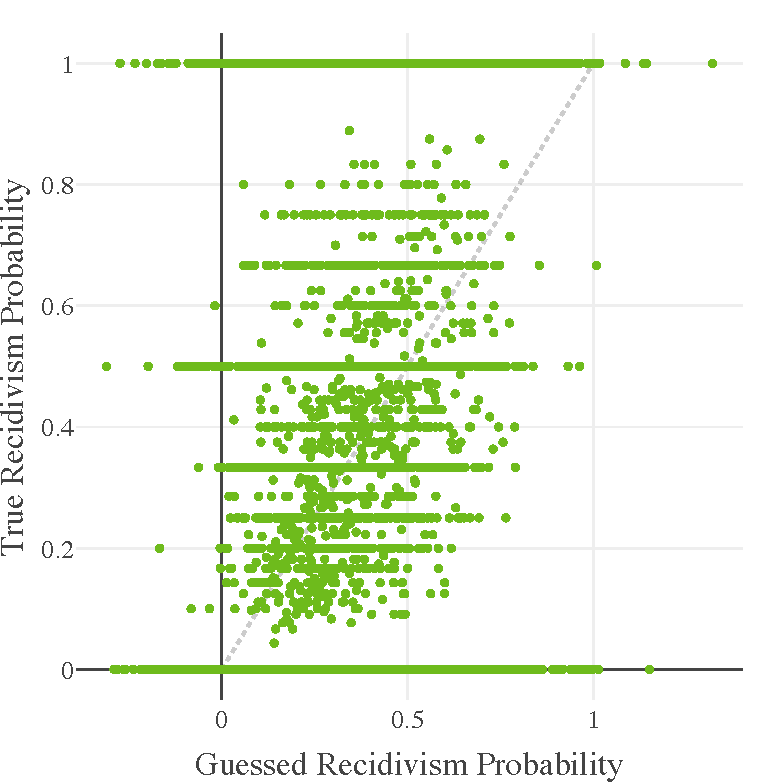
\includegraphics[width=2in,height=2in]{MLPRegressor_regression.pdf}} \vspace{3mm} \\
    \begin{tabular}{c|c}
        Min & 0.000 \\
        $25^{th}$ & 0.068 \\
        $50^{th}$ & 0.145 \\
        $75^{th}$ & 0.279 \\
        Max & 1.273 \\
    \end{tabular} &
    \begin{tabular}{|c l|}
      \hline
      0.147 & White - NH \\
      0.153 & Black - NH \\
      0.134 & White - H \\
      0.113 & AI or NA \\
      0.114 & Asian or PI \\
      \hline
    \end{tabular} \vspace{3mm} \\
  \end{tabular}

\end{tabular}

  \caption{These four plots show the true recidivism probability versus guessed recidivism probability for each of the regression techniques (except for Delaunay, explained in Section \ref{sec:results}). The top two regression algorithms make predictions based only on local data while the bottom two algorithms are global fitting techniques. The left vertical table beneath each figure displays the percentiles of absolute errors when predicting the probability of recidivism with that algorithm. The right table beneath each figure shows the median error in recidivism likelihood for those predictions which were over-estimated (false positives) broken down by race. The race abbreviations are the same as in figure \ref{fig:classification_performance}.}
  \label{fig:regression_performance}
\end{figure*}

Now we consider the outputs of the global and local algorithms on the regression task of predicting recidivism likelihood. figure \ref{fig:regression_performance} displays the outcomes for four of the five algorithms. The column arrangement of the models is intentional, noting that nearest neighbor and regression tree perform similarly while the Voronoi mesh and neural network also perform similarly. The prediction outcomes are promising, demonstrating that 50\% of recidivism likelihood predictions have less than a .15 absolute error. The largest discrepancy in false positive rate by race is observed to be the neural network (same as for classification).

The most notable result that can be observed in figure \ref{fig:regression_performance} is that the Voronoi Mesh (VM) algorithm that makes predictions based only on a local support of roughly $2d$ (\thomastilde{}100) points from data competes with the global fitting Multilayer Perceptron based on all data (\thomastilde{}20K) points. The benefit of using the VM to make predictions in ethically sensitive applications is that \textit{every} prediction has a manageable set of source data that can be used to describe how a prediction is produced. Addressing the two points mentioned in Section \ref{sec:introduction}, statistical tests can be run on these source data points to reduce prediction bias in desirable ways. Along with simplified statistical testing, the opportunity can be taken during any prediction to validate the source data and remove entries that are evidently outliers. Finally, this type of prediction opens up the possibility of a legal right to a representative sample from any predictive models used in official legal proceedings (such as predicting recidivism).

Results for Delaunay were the most theoretically promising, because of the guaranteed compactness of support (exactly $d+1$ source points for any prediction). Unfortunately, after two weeks of computation the Delaunay code was not able to compute predictions for the data. This suggests either a bug in the recently released Fortran code, or an unexpected geometric degeneracy in the data being used to make predictions. Regardless of the cause of slowdown, Delaunay results could not be collected for this experimentation and that is left to future attempts.

%% ===================================================================

\section{DISCUSSION (RB)}
\label{sec:discussion}

% will be fixing up this section once Thomas gets the final results in, email either the group or more specifically Reid once that's done!
    
% still waiting on dibiasing results until we can begin to question if our results are good enough    
    
For our experiments, we ran both condensed regression and full classification on all 3 of our models, with variation in the definition of Age either as a category or as a number. From these results, it is noted that interpretting age as a category or as a number will produce negligible differences in the results on the models. The condensed regression results were fairly similar between all 3 classifiers, with the largest number of guesses on recidivism being only 3\% more than the minimum. However, we ended up creating a 4th model for the Voronoi Mesh for condensed regression which happened to compete well with the Multilayered Perceptron Regressor.  Based off of this, we have instead decided to focus on all the models of full classification, but only focus on the Voronoi Mesh and Multilayered Perceptron Regressors in condensed regression.

\subsection{Full Classification}

As can be seen from our results in figure \ref{fig:classification_performance}, all of our models are at least 60\% correct in classifying the correct recidivism of individuals, with the Multilayered Perceptron resulting in the best classification rate at approximately 67\%. Notably, this model guessed nearly \textbf{half} as many recidivism candidates as the Nearest Neighbor algorithm, yet still achieved a better overall accuracy. This can likely be attributed to the fact that the \textit{true} recidivism for this dataset was actually only 33\%, meaning that guessing non-recidivism will be more likely to be correct.

In terms of interpretability, it's possible to see that for all 3 models that, regardless of the true accuracy, all of the models had a relatively even amount of bias when generating a false positive. One must also note that the Asian or Pacific Islander category was also the smallest population size by far, meaning that having the highest percentage of bias from false positives is expected for all 3 models. From these results, the Nearest Neighbor, Decision Tree, and Mulitlayered Perceptron have a false positive standard deviation of 2.03, 2.11, 2.32 from their mean respectively. This is well within a tolerable bias range considering that the more guesses on recidivism will result in a higher false positive rate overall. With this in consideration, the Nearest Neighbor, Decision Tree, and Multilayered Perceptron models ended up guessing recidivism 19.8\%, 11.6\%, and 7.8\% of the time, which follows our assumptions on the biases.

We can conclude from our initial set of tests that all of our models have been relatively debiased while also having a reasonable accuracy when guessing recidivism or non-recidivism. These findings aside, the best model that results in the least number of false positives as well as the highest accuracy is our Multilayered Perceptron model with a 67.7\% accuracy and average false positive rate of 6.8\%. Interestingly, this also coincides with the trend that less guesses on recidivism tended to result in better accuracy, with the Multilayerd Perceptron guessing recidivism half as much as the Nearest Neighbors Classifier.

\subsection{Condensed Regression}

In this section we are just focusing on the Voronoi Mesh and Multilayer Perceptron Regressors' results, since the other 2 models didn't produce enough positive results. From the results seen in figure \ref{fig:regression_performance}, the Voronoi Mesh has been able to produce results that compete quite well with that of the Multilayered Perceptron. This shows us that the local predictive models are able to produce just as good results as the global predictive models. In the case of the Nearest Neighbor and Decision Tree Regressors, not enough positive results in accuracy nor false positives meant that those models would not be as useful in classification of bias. 

One odd thing of note is that the Multilayered Perceptron Regressor tended to produce weird prediction by nature (which were outside of the usual range [0,1], which in it of itself is undesirable in our results. This is to be expected with this type of Regressor, but our hope would be that such things would not happen in most datasets as it could produce more exact results. Regardless of these oddities, the Multilayered Perceptron Regressor tended to produce quite minimal median error in recidivism likelihood for those predictions that were false positives (at least compared to that of the 2 less than satisfactory models). The Voronoi Mesh has similar results in its minimal median error as well as doesn't produce odd predictions outside of the usual range.

\subsection{Takeaways}

From these results, we can assume that it should be relatively possible to use these classifiers to ensure data is clean and relatively debiased. A very positive result shows that both Global Predictive \textbf{and} Local Predictive Models can be beneficial in locating bias within datasets and can guess well on recidivism rates without much bias. In the case when the false positive standard deviation is much larger than 2, we can assume then that there is a bias towards one or more races. We can therefore utilize these algorithms to ensure that a given dataset has not been ethically comprimised due to unintentional (or perhaps even intentional) biases. Similarly, we could use these classifiers as a means to figure out which features in a dataset are the cause of significant bias in the results by generating false positive rates for different combinations of features. This is on track with our expected results in producing an improvement to identify as well as clean bias either statistically or by human users on a per-prediction bias.

%% ===================================================================

\section{CONCLUSION (All members)}
\label{sec:conclusion}

This paper presents a comparative analysis of popular global predictive modeling algorithms and less popular local prediction techniques. Results demonstrate that algorithms which rely only on local support are capable of producing predictions of comparable (and sometimes superior) accuracy to those popular techniques while also maintaining an enhanced level of interpretability. The potential for operating under more concise legal definitions and meaningful statistical analyses further supports the implementation of explainable prediction methodologies. This recidivism case study demonstrates that the use of more explainable models could not only strengthen the ethical application of data science, but also make the process of cleaning and validating data manageable in the long term.


%% ===================================================================

\section{ACKNOWLEDGEMENTS \& CONTRIBUTIONS}

The data for this project was collected from the \texttt{data.gov} project called "3-year-recidivism-for-offenders-released-from-prison" provided by the State of Iowa.

\vspace{5mm}

All of the code for this project is available at \\
\texttt{https://github.com/tchlux/GRAD\_5134\_Project}

\vspace{5mm}

\begin{tabular}{l|l}
  \textbf{Component} & \textbf{Primary Contributer} \\ \hline
  Abstract and Conclusion & All Members \\
  Introduction & Mohammed Almanaa \\
  Related Work & Stefan Nagy \\
  Data & Sirui Yao \\
  Results + Code & Thomas Lux \\
  Discussion & Reid Bixler \\
\end{tabular}

\vspace{5mm}

\bibliographystyle{acm-ref-format}
\bibliography{paper}

\end{document}
